\documentclass[11pt]{article}
\usepackage[margin=1in]{geometry}
\usepackage{graphicx}
\usepackage{microtype}
\usepackage{verbatim}
\usepackage{amsmath}
\usepackage{nicefrac}
\usepackage[colorlinks=false, hidelinks]{hyperref}
\usepackage{caption}
\usepackage{subcaption}
\usepackage{listings}
\usepackage{harmony}
\usepackage{wasysym}

\begin{document}

\title{Tricycle Lights\\Embedded System Design, Lab 6}
\date{October 29, 2015}
\author{Ben Lorenzetti}
\maketitle

\tableofcontents

\clearpage

\section{Objectives and Problem Description}
\label{problem-specs}

\subsection{Tricycle Lights}

Blink two LEDs, representing left and right turn signals,
depending on the position of a rotary potentiometer,
which represents a steering wheel. The following conditions should be met.

\begin{enumerate}
\item
Use the potentiometer and LEDs on the 44--Pin Demo Board.
\item
Use the LED connected to RD7 for the left turn signal, and RD0 for right.
\item
When wheel is in neutral position (wiper in middle of pot.),
both turn indicator lights should be off.
\item
When turned counterclockwise or clockwise from neutral position,
the left or right LEDs should blink at a rate proportional to the
angular displacement from neutral position.
\end{enumerate}

\section{Procedure}

\subsection{Potentiometer and LEDs on the 44--Pin Demo Board}

\begin{figure}
\centering
	\begin{subfigure}[b]{.3\textwidth}
		\centering
		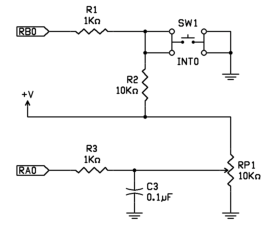
\includegraphics[width=\textwidth]{Figures/demo-board-pot-pushbutton-circuit.pdf}
		\caption[]%
		{{\small Potentiometer Input}}
	\end{subfigure}
	\quad
	\begin{subfigure}[b]{0.3\textwidth}
		\centering
		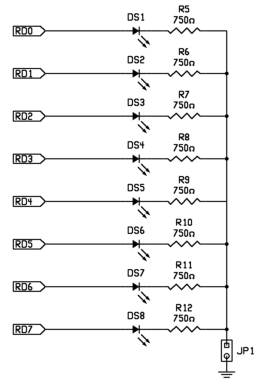
\includegraphics[width=\textwidth]{Figures/demo-board-led-circuit.pdf}
		\caption[]%
		{{Output LEDs}}
	\end{subfigure}	
	\caption{I/O Circuit Diagrams from the 44--Pin Demo Board User's Manual}
	\label{io-circuit-diagram}
\end{figure}

In this lab, we will need to measure a potentiometer input (the steering wheel)
and blink two LEDs for output. The 44--pin demo board for the PIC16F887
has all of this hardware on board. The potentiometer and LEDs are connected to
pins as shown in the circuit diagram in
\hyperref[io-circuit-diagram]{figure \ref{io-circuit-diagram}}.

According to the specifications, the LED at RD7 should be the left blinker
and the LED at RD0 should be the right blinker.

\subsection{Clock Sources on the PIC16F887 and 44--Pin Demo Board}
\label{clock-sources-section}

To use the analog to digital converter, we need to know the frequency of
the system's clock. The PIC16F887 microcontroller can be configured to
use an internal RC oscillator or external crystals/clocks with various
prescalars. The block diagram below shows all of the possible options
for the oscillator module of the PIC16F887.

\begin{center}
	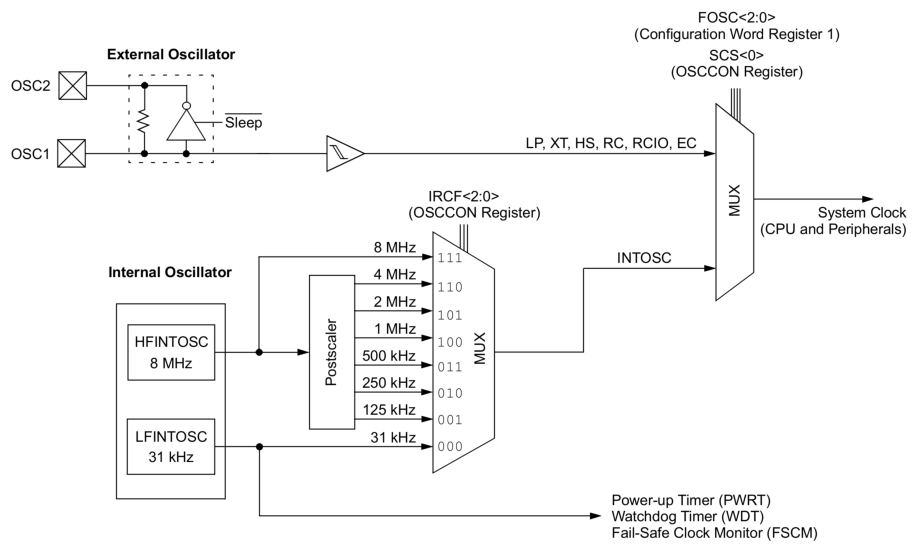
\includegraphics[width=0.8\textwidth]{Figures/pic16f887-clock-sources-diagram.pdf}
	\captionof{figure}{Oscillator Module Block Diagram from PIC16F887 Datasheet}
\end{center}

\begin{figure}
	\centering
	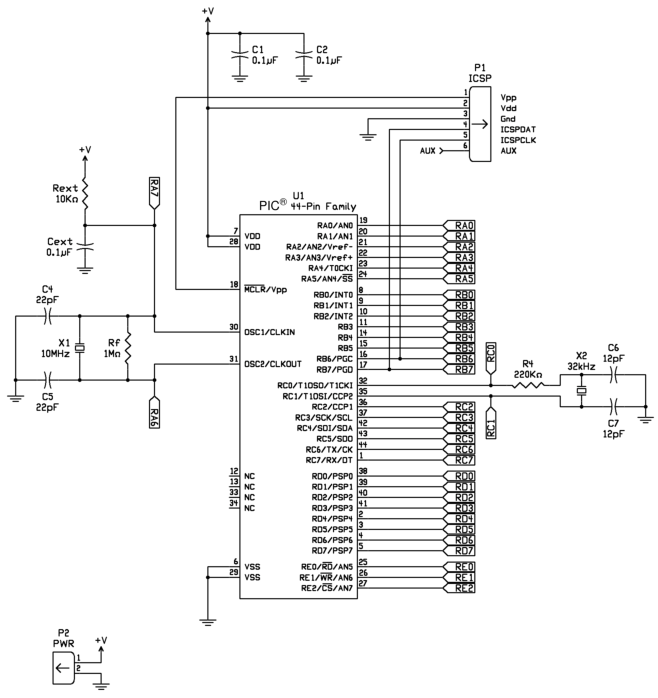
\includegraphics[width=1\textwidth]{Figures/demo-board-clock-power-programming-circuit.pdf}
	\captionof{figure}{Oscillators, Power, and Programming Connections on the 44--Pin Demo Board}
	\label{demo-board-oscillators-circuit}
\end{figure}

The 44--pin demo board has 10 MHz and 32 kHz oscillators, which are connected to the
$\mu$Controller as shown in
\hyperref[demo-board-oscillators-circuit]{figure \ref{demo-board-oscillators-circuit}}.
However, by default the PIC16F887 $\mu$Controller runs from its internal high frequency RC oscillator
with the prescalar set to yield a 4 MHz clock rate.
\begin{equation*}
F_{OSC}=4MHz
\end{equation*}

\subsection{PIC16F887 Analog to Digital Converter (ADC)}

\begin{figure}
	\centering
	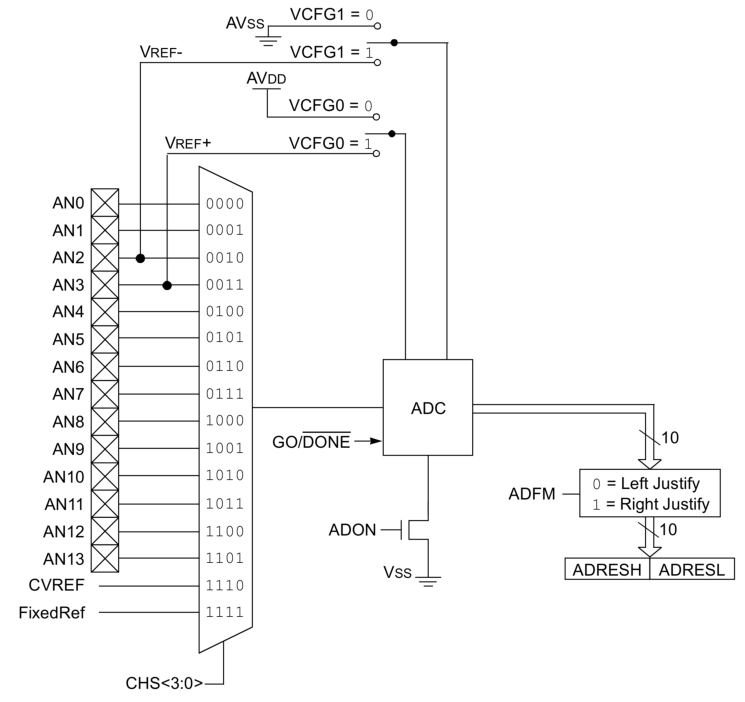
\includegraphics[width=0.6\textwidth]{Figures/pic16f887-adc-block-diagram.pdf}
	\caption{PIC16F887 ADC Block Diagram}
	\label{pic16f887-adc-block-diagram}
\end{figure}

The PIC16F887 has a successive approximation analog to digital converter (ADC)
which can be used to measure the voltage on \texttt{RA0} with 10--bit precision.
\hyperref[pic16f887-adc-block-diagram]{Figure \ref{pic16f887-adc-block-diagram}} and
from the the PIC16F887 datasheet shows how the ADC fits into the $\mu$Controller.

\begin{figure}
	\centering
	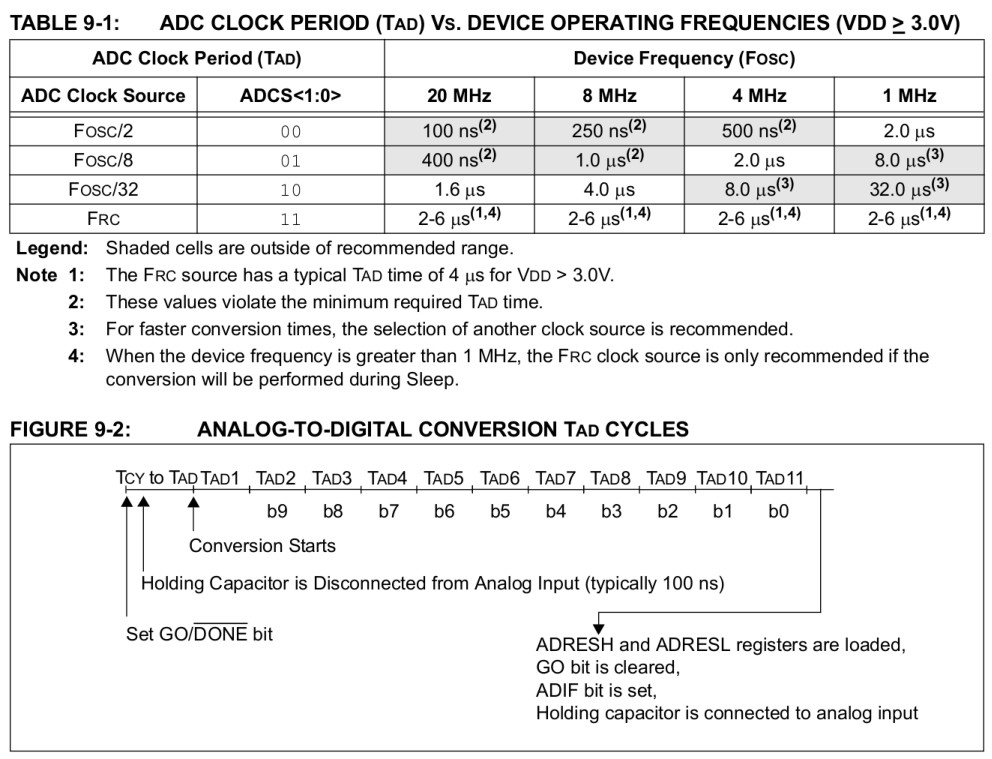
\includegraphics[width=0.7\textwidth]{Figures/pic16f887-adc-clock-sources-and-conversion-time.pdf}
	\caption{PIC16F887 Recommended ADC Clock Rate ($T_{AD}$) and Measurement Time}
	\label{pic16f887-adc-clock-sources-and-conversion-time}
\end{figure}

Successive approximation is a process similar to binary search, where the input
voltage being measured is compared with a series of binary decisions honing
in on the actual value. The ADC has its own clock source, but usually it is
just the main CPU/peripherals clock divided by a prescalar. The ADC requires
$11*T_{AD}$ to complete one conversion: 10 ADC clock cycles for 10 binary
comparisons with 1 more ADC clock cycle in overhead.
\hyperref[pic16f887-adc-clock-sources-and-conversion-time]{Figure
\ref{pic16f887-adc-clock-sources-and-conversion-time}}, from the PIC16F887
datasheet, shows the 11--step conversion process and the recommended
prescalar from the main CPU clock.

The ADC clock $T_{AD}$ should not exceed the recommended rate because parasitic
capacitance in the pins and traces will cause aliasing.
In \hyperref[clock-sources-section]{section \ref{clock-sources-section}},
we decide the main CPU clock ($F_{OSC}$) is 4 MHz;
therefore, the prescalar \texttt{ADCS} should be
\emph{configured to $F_{OSC/8}$}:
\begin{equation*}
\textrm{\texttt{ADCON0}}=\textrm{01XX XXXX}
\end{equation*}

The result of an ADC operation is stored in registers \texttt{ADRESH} and
\texttt{ADRESL} and is equal to
\begin{equation*}
\textrm{\texttt{[ADRESH:ADRESL]}}=\frac{2^{\textrm{bit precision}}-1}{V_{\textrm{REF+}}-V_{\textrm{REF+}}}*V_{in}
\end{equation*}

For this lab, a human would not be able to notice the difference between 10--bit precision
and 8--bit precision in the small angular range of the rotary potentiometer.
Furthermore, because the PIC16F887 uses an 8--bit data paradigm,
reducing the ADC result to eight bits would make implementation much easier.
This can be done by \emph{configuring the ADC to justify left} and then taking only \texttt{ADRESH}.
\begin{equation*}
\textrm{\texttt{ADCON1}}=\textrm{0XXX XXXX}
\end{equation*}

According to the schematic in \hyperref[io-circuit-diagram]{figure \ref{io-circuit-diagram}},
the $10k\Omega$ potentiometer has terminals connected to \texttt{V+} and \texttt{Gnd};
and its wiper is connected to \texttt{RA0} (\texttt{PORTA, 0}) with a $1k\Omega$ current limiter.
With this configuration, the voltage from the wiper can vary between $V_{SS}$ and $V_{DD}$.
The ADC can be \emph{configured to the upper and lower bounds of the expected input} for
more accurate measurments. For $V_{SS}$ and $V_{DD}$, \texttt{VCFG[1:0]} should be
\begin{equation*}
\textrm{\texttt{ADCON1}}=\textrm{XX00 XXXX}
\end{equation*}

With these configuration settings, the result of an ADC conversion is now stored in
\texttt{ADRESH} and given by
\begin{equation*}
\textrm{\texttt{ADRESH}}=\frac{255}{3.3V}*V_{in}
\end{equation*}

The general process for ADC conversion in code is:
\begin{enumerate}
\item Configure Port\\
	\texttt{BANKSEL  TRISA}\\
	\texttt{BSF      TRISA, 0	; set RA0 to input}\\
	\texttt{BANKSEL  ANSEL}\\
	\texttt{BSF      ANSEL, 0	; set RA0 to analog}
\item Configure ADC Module\\
	\texttt{; ADCON1 = 0xxx xxxx}	- select result format as left justify\\
	\texttt{; ADCON1 = xx00 xxxx}	- configure reference voltages to $V_{SS}$ and $V_{DD}$\\
	\texttt{; ADCON0 = 01xx xxxx}	- set ADC conversion clock rate to $F_{OSC/8}$\\
	\texttt{; ADCON0 = xx00 00xx}	- select input channel to AN0\\
	\texttt{; ADCON0 = xxxx xxx1}	- turn ADC on
	\texttt{BANKSEL  ADCON1}\\
	\texttt{MOVLW    B'00000000'}\\
	\texttt{MOVWF    ADCON1}\\
	\texttt{BANKSEL  ADCON0}\\
	\texttt{MOVLW    B'01000001}\\
	\texttt{MOVWF    ADCON0}\\
\item Configure ADC interupt (optional)
\item Wait for the required ADC settling time
\item Start conversion by setting the $\textrm{GO}/\overline{\textrm{DONE}}$ bit\\
	\texttt{BSF      ADCON0, GO     ; start conversion}
\item Wait for ADC conversion to complete\\
	\texttt{BTFSC    ADCON0, GO     ; is conversion done?}\\
	\texttt{GOGO     \$-1           ; if no, test gain}
\item Read the ADC result from \texttt{ADRESH} (and \texttt{ADRESL})
\end{enumerate}

\subsection{Implementation Flowchart}

\subsection{Delay Function}

\subsection{Linear Mapping}

\section{Expected Results}

\section{Experiment and Design Revisions}

\subsection{Command Line Assembly}

My \texttt{.asm} source files were assembled on the command line so
please do this if they don't compile nicely in the IDE.
On Ubuntu, with the default MPLAB installation location, 
from the directory containting \texttt{tricycle-lights.asm}, the commands are:
\begin{verbatim}
$ cp /opt/microchip/mplabx/v3.10/mpasmx/p16f887.inc ./p16f887.inc
$ /opt/microchip/mplabx/v3.10/mpasmx/mpasmx -p16f887 tricycle-lights.asm
$ more tricytle-lights.ERR
\end{verbatim}

\section{Observations}

\begin{center}
	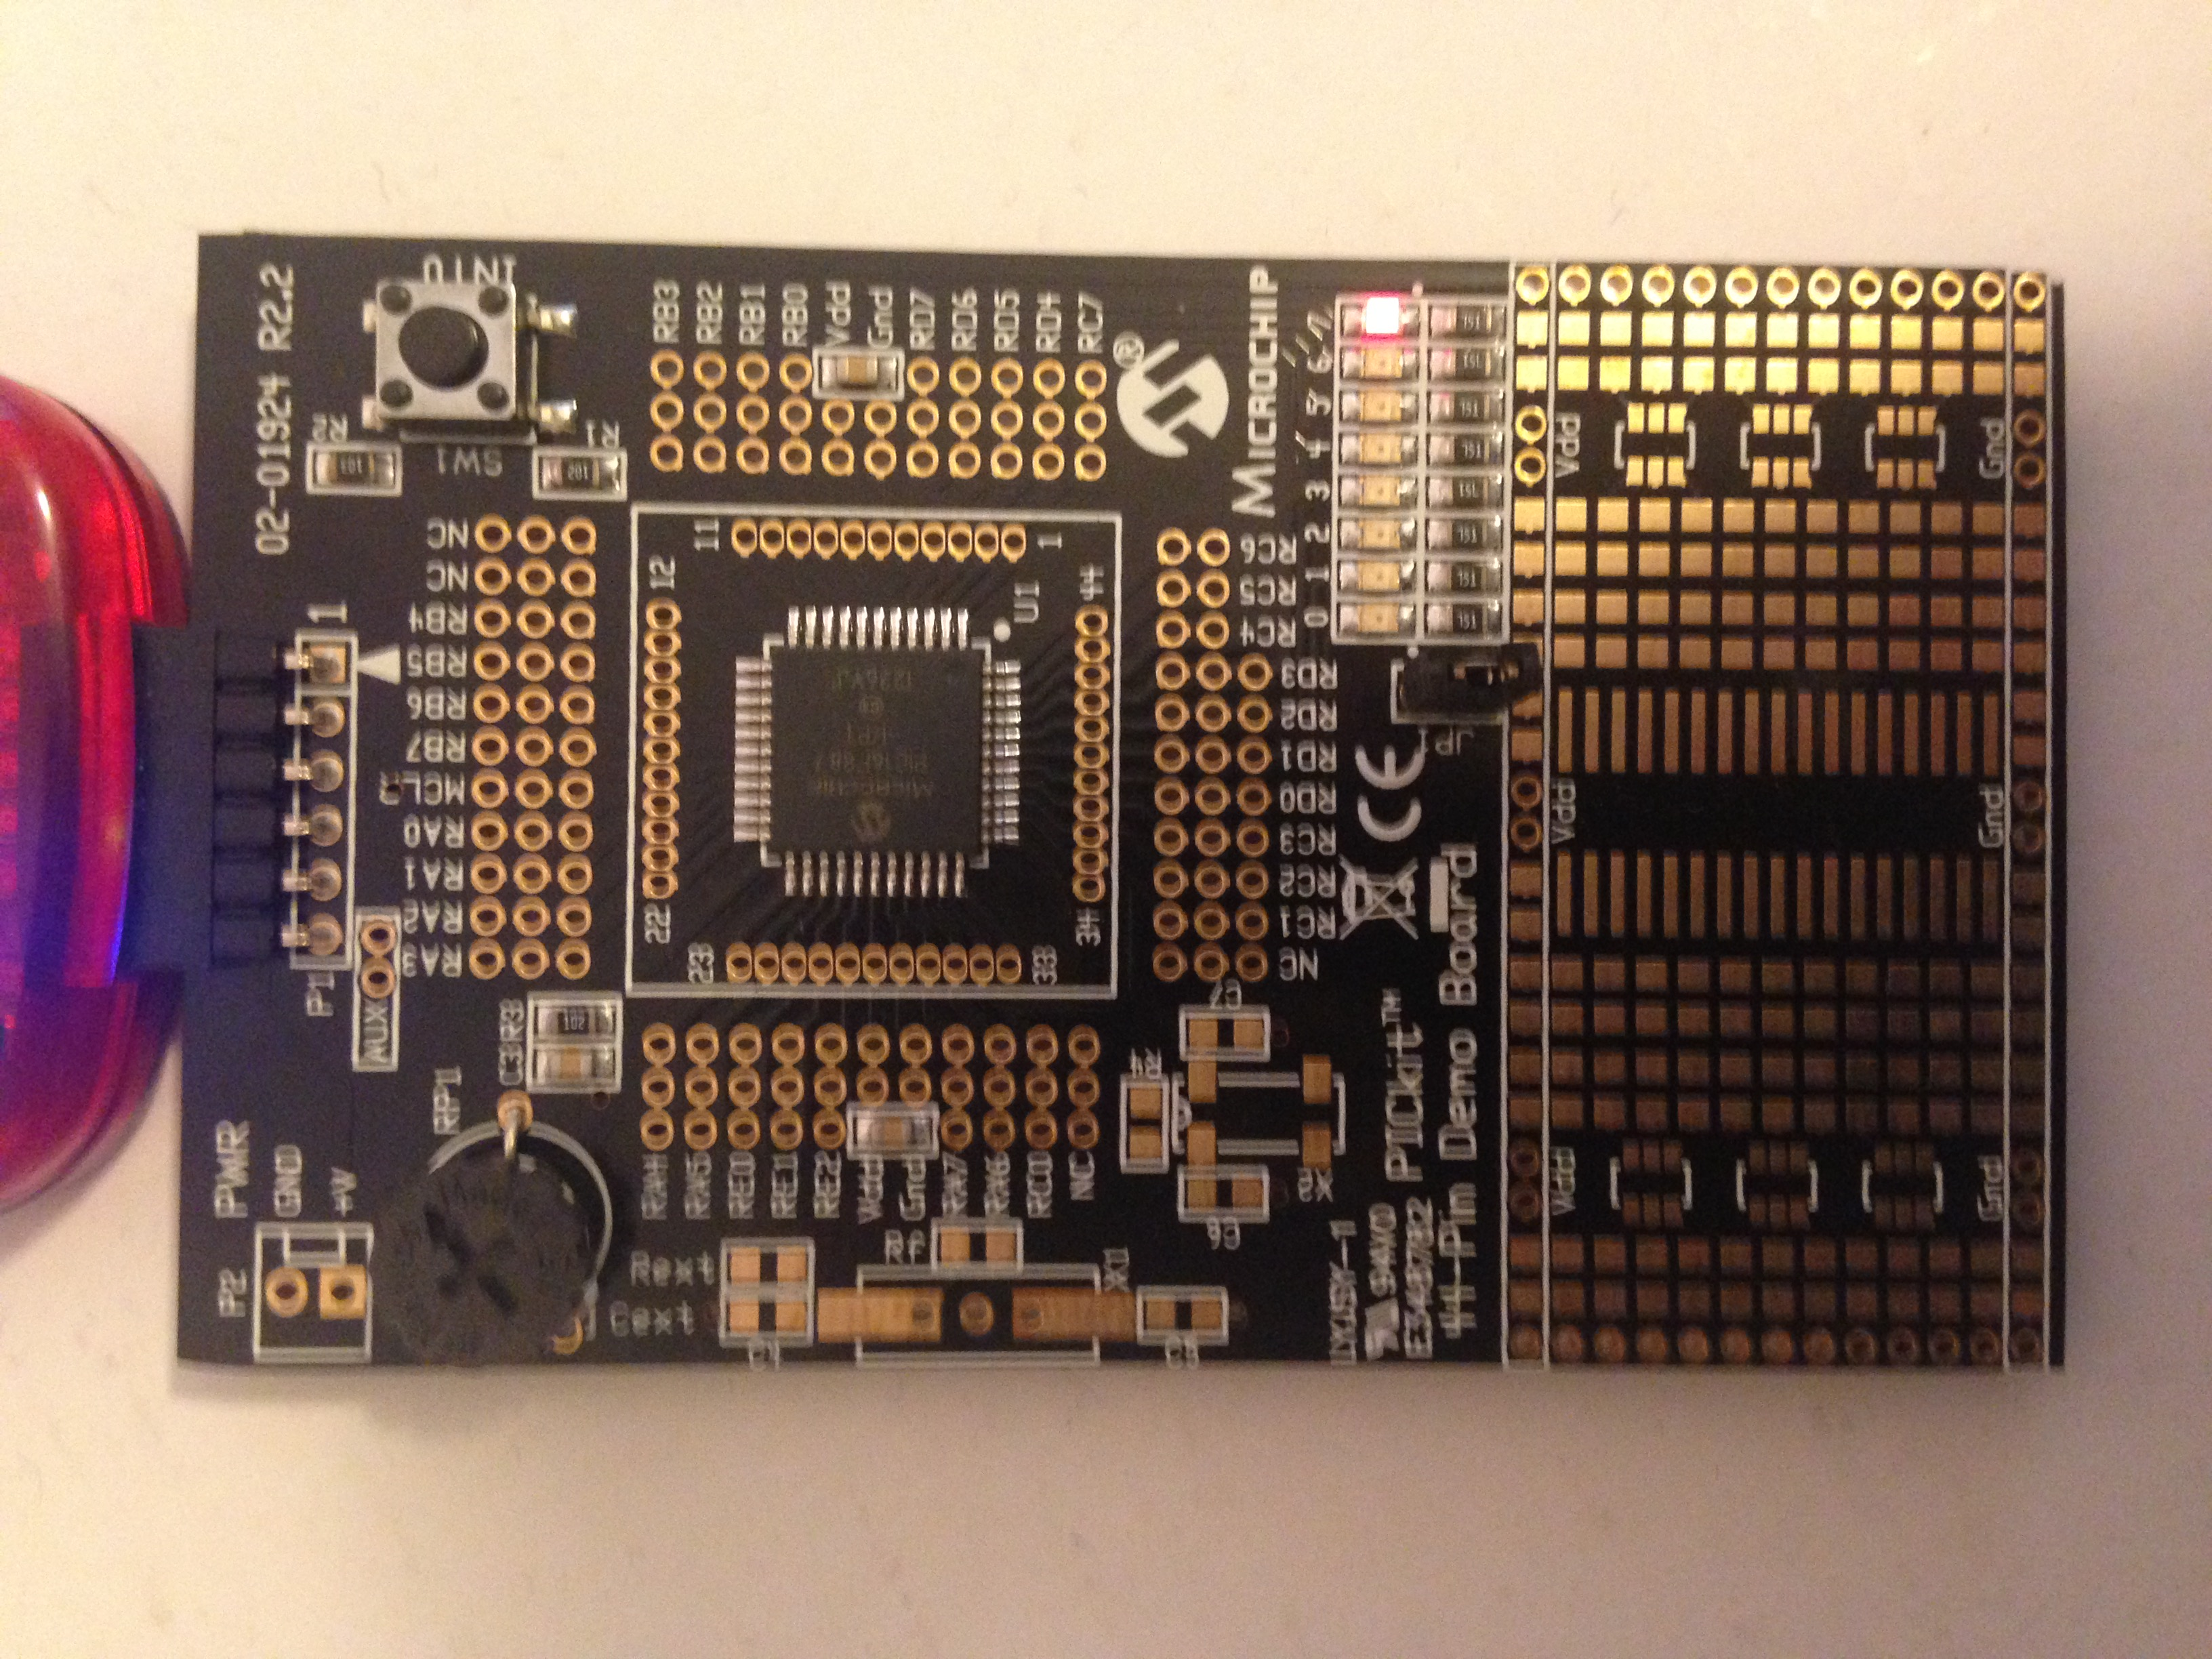
\includegraphics[width=0.5\textwidth]{Figures/demo.jpeg}
	\captionof{figure}{Demonstration of Tricycle Turn Lights}
	\label{tricycle-lights-jpg}
\end{center}

\section{Discussion}

\clearpage

\section{Tricycle Lights Implementation Code}
\label{implementation-code}

\lstinputlisting[breaklines, basicstyle=\small]{Tricycle-Lights/tricycle-lights.asm}

\end{document}
